\documentclass{article}
\usepackage{graphicx}
\usepackage{polski}
\usepackage[utf8]{inputenc}
\usepackage[french,polutonikogreek,polish]{babel}
\usepackage{csquotes}
\begin{document}
\section{Porównanie funkcji haszującej} \label{p1}
	Porównanie dotyczy zbioru liczb całkowitych z zakresu $x \in \{0,1,2,\ldots,10^4 - 1\}$ oraz wielkości tablicy haszującej równej $a = 100$. Porównywane są 3 metody z czego dwie między sobą różnią się sposobem zaokrąglania wyniku. Zaokrąglanie w metodzie środka kwadratu jest wykorzystywane w celu jednoznacznego określenia początku sekwencji wynikowej. Metody:
	\begin{enumerate}
		\item metoda środka kwadratu(zaokrąglanie przedziału w górę),
		\item metoda środka kwadratu(zaokrąglanie przedziału w dół),
		\item metoda 'sumowania przesunięć bitowych'.		
	\end{enumerate}
	\begin{figure}[h]
		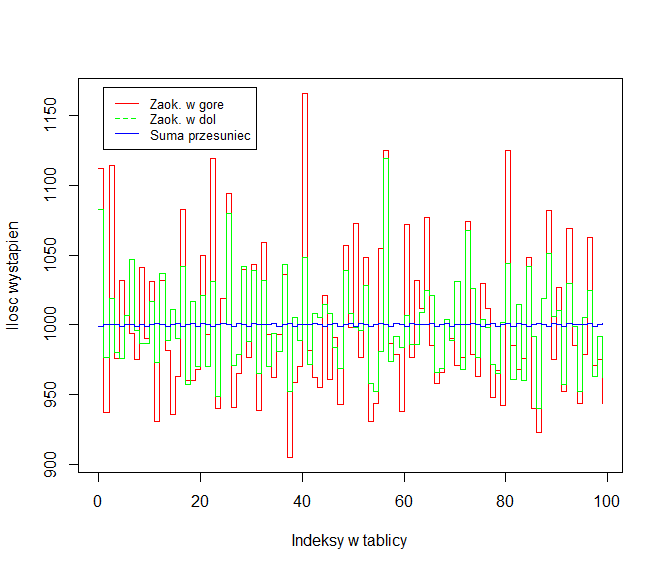
\includegraphics[width=\linewidth]{1.png}
		\caption{Porównanie funkcji haszujących dla $x \in \{0,1,2,\ldots,10^4 - 1\}$ oraz rozmiaru tablicy haszującej $a = 100$.}
	\end{figure}
	\paragraph{Wnioski}	
	Metoda środka kwadratu osiaga bardzo niejednolite wyniki. Odchylenia standardowe dla takiej funkcji haszującej wynosi odpowiednio $53.76999$ oraz $32.64347$ dla zaokrąglania w górę i w dół. Natomiast metoda sumowania przesunięć bitowych posiada bardzo małe odchylenie równe zaledwie $0.7385489$. 

\section{Porównanie funkcji haszującej dla wariancji z powtórzeniami}
	W poniższym paragrafie opisane zostaną wyniki wcześniej wspomnianych funkcji dla wariancji cztero-elementowych($k = 4$) z powtórzeniami dla alfabetu łacińskiego($x \in \{A,\ldots,Z\}$).
	%\subsection{Sposoby wyznaczania liczby z ciągu symboli}	
		\subsection{I Sposób wyznaczania liczby z ciągu symboli}\label{p2}
			Wyznaczanie liczby z ciągu symboli odbywa się poprzez tworzenie liczby w zapisie dziesiętnym, gdzie współczynnikami kolejnych potęg są wartości kodów ASCII poszczególnych symboli --- $L =$'A'$*10^3+$'B'$*10^2+$'C'$*10+$'D'.
			
			\begin{figure}[h]
				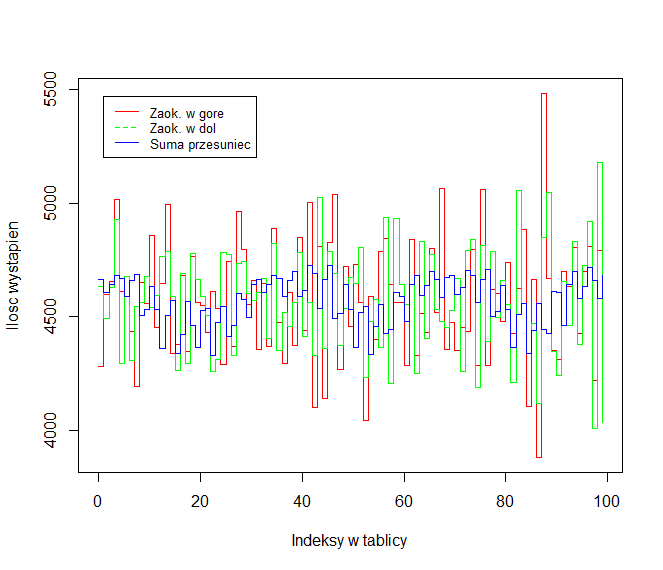
\includegraphics[width=\linewidth]{2.png}
				\caption{Porównanie f. haszujących dla I sposobu.}
			\end{figure}		
			Tabela \ref{sp1} zawiera odchylenia standardowe dla uzyskanych histogramów:
			
			\begin{table}
				\centering
				\label{sp1}
				\caption{Odchylenia standardowe dla I sposobu}
				\begin{tabular}{|c|c|}
					\hline
					Metoda & Odchylenie standardowe \\\hline\hline 
					środka kwadratu(góra)& $258.9582$ \\\hline  
					środka kwadratu(dół)	& $233.916$ \\\hline  
					sumowania przesunięć bitowych & $103.8099$\\\hline 
				\end{tabular} 
			\end{table}
						
			\paragraph{Wnioski}
		Metoda sumowania przesunięć bitowych okazała się podobnie jak w poprzenium przypadku dużo lepsza. 
		\subsection{II Sposób wyznaczania liczby z ciągu symboli}\label{p3}
			Ciąg symboli wyznaczany jest poprzez dodawanie oraz przesuwanie bitowe kolejnych wartości kodów ASCII ciągu symboli do wartości początkowe równej zero. 
			\begin{figure}[h]
				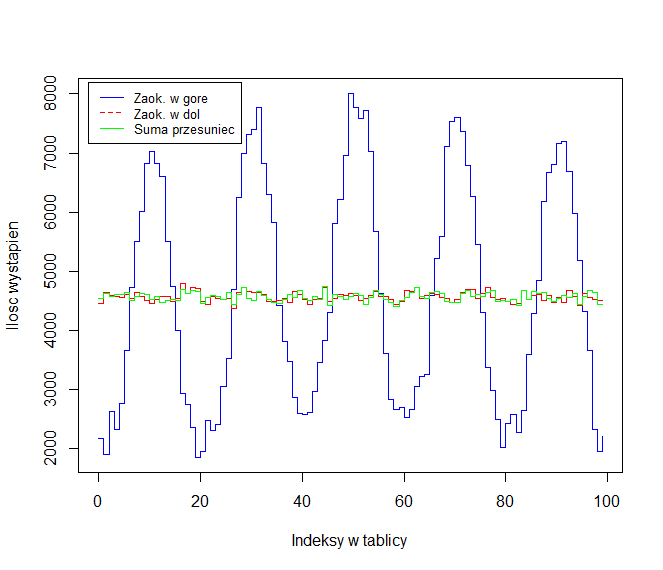
\includegraphics[width=\linewidth]{3.png}
				\caption{Porównanie f. haszujących dla II sposobu.}
			\end{figure}
			Tabela \ref{sp2} zawiera odchylenia standardowe dla uzyskanych histogramów:
			\begin{table}
			\centering
			\label{sp2}
			\caption{Odchylenia standardowe dla II sposobu}
			\begin{tabular}{|c|c|}					
				\hline
				Metoda & Odchylenie standardowe \\\hline\hline 
				środka kwadratu(góra)& $80.8298$ \\\hline  
				środka kwadratu(dół)	& $77.59492$ \\\hline  
				sumowania przesunięć bitowych & $1926.456$\\\hline 								
			\end{tabular} 		
			\end{table}
			
			\paragraph{Wnioski}
			Zmiana sposób wyznaczania liczby z ciągu symboli wpłyneła znacząco na zachowanie się poszczególnych funkcji haszujących. Tym razem prosta metoda środka kwadratu uzyskała dużo lepsze wyniki.
			
\section{Podsumowanie}
W pierwszym paragrafie(\ref{p1}) metoda sumowania przesunięć bitowych dała najlepszy rezultat ponieważ wartości cechowały się jednostajnym rozkładem prawdopodobieńtswa. Jeżeli mamy do czynienia z niejednostajnym rozkładem prawdopodobieństwa jak w przypadku wariancji z powtórzeniami dla alfabetu bardzo istotne jest dobranie dwóch elementów: funkcji przekształcającej(w przykładzie omówionym w paragrafie \ref{p2} -- ciąg symboli w liczbę) oraz funkcji haszującej. Zmiana funkcji omówiona w paragrafie \ref{p3} przekształcania ciągu symboli bardzo wpłyneła na jakość funkcji haszującej ponieważ generowane indeksy zbyt często się powtarzały, dlatego wykorzystanie tablicy haszującej nie było równomierne. W rezultacie metoda środka kwadratu dla zmodyfikowanej funkcji przekształcania okazała się lepsza i posiadała mniejsze odchylenie od wartości średniej.

\section{Użyte programy}
\begin{itemize}
	\item Java - jako język programowania do generowania wyników
	\item R - język i środowisko do generowania wykresów i wyznacznia odchyleń
\end{itemize}
\end{document}